\subsection{Среда LunarLander}

Среда LunarLander впервые упоминается в пакете сред Gym \cite{towers2025gymnasiumstandardinterfacereinforcement}, которая представляет собой задачу управления в условиях двумерной физической симуляции с непрерывным пространством состояний. Задача когнитивного агента заключается в осуществлении безопасной и мягкой посадки космического модуля на заданную посадочную площадку, расположенную между двумя маркерными флажками. В отличие от задачи балансировки маятника, здесь агент должен научиться преодолевать гравитацию и управлять инерцией, аккуратно дозируя тягу главного и двух маневровых двигателей.

В рамках данного исследования для оценки способности алгоритмов к обобщению устойчивости тестирование проводилось в двух различных конфигурациях среды: в условиях идеального вакуума и с применением сильного бокового ветра и турбулентности. Сравнительный анализ влияния этих возмущающих факторов на стабильность агентов подробно рассматривается в разделе экспериментальных результатов.

\begin{figure}[h!] % [h!] - попытка разместить картинку "здесь" (here)
  \centering
  
  % 0.7 от ширины текста страницы (0.7\textwidth)
  % Замени 'cartpole_env.png' на реальное имя твоего файла, если оно другое.
  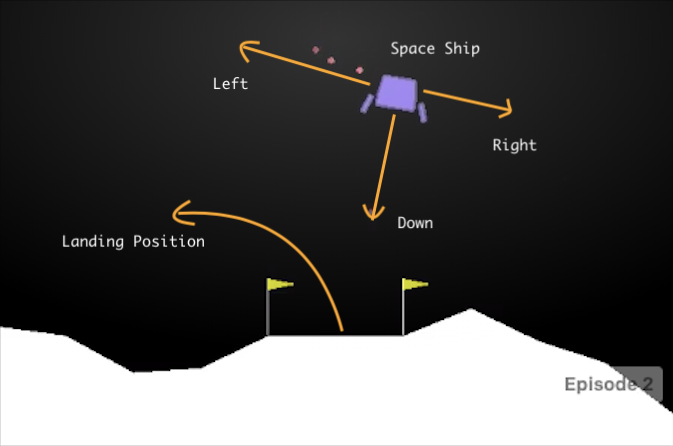
\includegraphics[width=0.6\textwidth]{./images/lunarlander.png}
  
  \caption{Вид среды LunarLander.}
  \label{fig:lunarlander_scheme}
\end{figure}


\subsubsection{Пространство состояний}

Сенсорный аппарат агента передает вектор наблюдений, состоящий из 8 числовых параметров, исчерпывающе описывающих текущее кинематическое состояние модуля:

\begin{itemize}

  \item \textbf{Позиция центра масс} аппарата в двумерной системе координат ($x, y$).

  \item \textbf{Вектор линейной скорости} перемещения модуля по осям $x$ и $y$.

  \item \textbf{Угол наклона (крена)} аппарата относительно идеальной вертикали.

  \item \textbf{Угловая скорость} вращения модуля.

  \item \textbf{Два дискретных булевых флага}, сигнализирующих о наличии физического контакта левой и правой посадочных опор с поверхностью.

\end{itemize}

\subsubsection{Пространство действий}

Пространство возможных решений агента является дискретным и состоит из 4 взаимоисключающих команд, выбираемых нейросетью на каждом такте симуляции:

\begin{itemize}

  \item \textbf{0:} Не предпринимать никаких действий (свободное падение).

  \item \textbf{1:} Включить левый маневровый двигатель (для корректировки крена вправо).

  \item \textbf{2:} Включить главный (нижний) маршевый двигатель.

  \item \textbf{3:} Включить правый маневровый двигатель (для корректировки крена влево).

\end{itemize}

\subsubsection{Функция награды и условия завершения}

В отличие от бинарного сигнала выживания в CartPole, функция приспособленности в LunarLander имеет сложную композитную структуру, стимулирующую достижение цели при максимальной экономии ресурсов:

\begin{itemize}

  \item За успешное касание поверхности обеими опорами агенту начисляется бонус в +100 очков.

  \item За движение к центру целевой площадки и корректное снижение скорости присуждается от +100 до +140 очков.

  \item В случае крушения модуля (падения на корпус) накладывается строгий штраф в размере -100 очков.

  \item Работа двигателей пенализируется для оптимизации расхода топлива: каждый такт работы главного двигателя стоит -0.3 очка , а использование боковых маневровых двигателей штрафуется на -0.03 очка за такт.

\end{itemize}

Один эпизод симуляции принудительно обрывается при достижении лимита в 1000 шагов, а также при успешной посадке или крушении модуля. Идеальная, мягкая посадка в центр площадки позволяет набрать около 250–300 очков. Официальным порогом успешного решения среды, свидетельствующим о сходимости алгоритма, считается достижение средней награды в 200 баллов.

\subsubsection{Конфигурация алгоритма NEAT для LunarLander}

\href{https://github.com/Isn0v/neat-training/blob/master/environments/lunar-lander/neat/neat.cfg}{Файл конфигурации NEAT}\footnote{\url{https://github.com/Isn0v/neat-training/blob/master/environments/lunar-lander/neat/neat.cfg}} определяет фундаментальные правила эволюции. Ниже приведены ключевые параметры, использованные в экспериментах:


\paragraph{Основные параметры популяции и завершения:}
  \begin{itemize}

    \item \textbf{Размер популяции (pop\_size = 150):} Данный параметр устанавливает количество нейронных сетей в каждом поколении. Значение 150 выбрано для обеспечения достаточного разнообразия геномов и эффективного поиска в пространстве решений.

    \item \textbf{Критерий приспособленности (fitness\_criterion = max):} Эволюция стремится максимизировать функцию приспособленности, выбирая лучшие геномы для размножения.

    \item \textbf{Порог приспособленности (fitness\_threshold = 200.0):} Обучение считается завершенным, если хотя бы один агент набирает 200.0 очков (стандартный порог решения среды).

  \end{itemize}

\paragraph{Архитектура и инициализация генома:}

  \begin{itemize}

    \item \textbf{Входы и Выходы:} Количество входных нейронов (num\_inputs = 8) и выходных нейронов (num\_outputs = 4) жестко зафиксировано и соответствует спецификации среды LunarLander.

    \item \textbf{Начальные скрытые слои (num\_hidden = 0):} Поиск начинается с самых простых сетей, без скрытых нейронов, чтобы позволить алгоритму NEAT самостоятельно развить сложную топологию.

    \item \textbf{Функции активации (activation\_default = tanh):} Все нейроны используют функцию активации гиперболического тангенса, которая позволяет вводить нелинейность в работу сети и выдает значения в диапазоне [-1, 1], что подходит для управления двигателями.

    \item \textbf{Начальные связи (initial\_connection = full\_direct):} На старте каждый входной нейрон соединен со всеми выходными нейронами, что обеспечивает минимальную функциональность сети.

  \end{itemize}

\paragraph{Вероятности мутации:}
  \begin{itemize}

    \item \textbf{Мутация весов (weight\_mutate\_rate = 0.8):} С вероятностью 80\% вес существующей связи будет изменен. Высокое значение стимулирует постоянное уточнение "тонкой настройки" управления.

    \item \textbf{Добавление нейрона/связи (node\_add\_prob = 0.2, conn\_add\_prob = 0.5):} Задают вероятности добавления нового скрытого нейрона (20\%) или новой синаптической связи (50\%). Это обеспечивает рост сложности топологии сети.

    \item \textbf{Удаление нейрона/связи (node\_delete\_prob = 0.2, conn\_delete\_prob = 0.5):} Задают вероятности удаления нейронов или связей, что позволяет упрощать избыточные структуры.

  \end{itemize}

\paragraph{Специация и эволюция популяции:}
  \begin{itemize}

    \item \textbf{Видообразование (compatibility\_threshold = 3.0):} Порог совместимости $\delta$ в 3.0 очка определяет, насколько генетически различными должны быть сети, чтобы считаться разными видами.

    \item \textbf{Застой видов (max\_stagnation = 20):} Если лучшая приспособленность вида не улучшается в течение 20 поколений, он считается застойным и не получает ресурсов для размножения. Это предотвращает "зацикливание" эволюции на локальных максимумах.

    \item \textbf{Элитизм (species\_elitism = 2):} Два лучших вида популяции защищены от удаления даже при застое.

    \item \textbf{Воспроизводство (elitism = 2, survival\_threshold = 0.2):} В каждом виде два лучших генома гарантированно выживают, и только 20\% наиболее приспособленных особей вида получают право на размножение.

  \end{itemize}


\subsubsection{Архитектура и гиперпараметры агента DQN для среды LunarLander}

Программная реализация алгоритма DQN для задачи посадки лунного модуля базировалась на фреймворке \texttt{stable\_baselines3}, рассмотренном в работе \cite{stable_baselines3}. Он предоставляет оптимизированные и надежные реализации современных алгоритмов обучения с подкреплением. В связи с необходимостью комплексной оценки устойчивости когнитивных агентов, обучение проводилось в два этапа: формирование \href{https://github.com/Isn0v/neat-training/blob/master/environments/lunar-lander/rl/model.py}{базовой политики управления}\footnote{\url{https://github.com/Isn0v/neat-training/blob/master/environments/lunar-lander/rl/model.py}} и \href{https://github.com/Isn0v/neat-training/blob/master/environments/lunar-lander/rl/model_windy.py}{универсальной политики}\footnote{\url{https://github.com/Isn0v/neat-training/blob/master/environments/lunar-lander/rl/model_windy.py}} в условиях ветренности.

Процесс Q-обучения регулировался следующим набором гиперпараметров:

\begin{itemize}

  \item \textbf{Буфер воспроизведения опыта:} Емкость буфера составила 100 000 переходов, что обеспечило эффективную декорреляцию обучающей выборки. Процесс обучения инициировался после накопления первых 1 000 случайных шагов (learning\_starts = 1000).

  \item \textbf{Оптимизация и градиентный спуск:} Использовался размер пакета данных равный 128. Скорость обучения была установлена на уровне $10^{-3}$.

  \item \textbf{Параметры обновления:} Дисконтирующий множитель $\gamma$ составил 0.99, ориентируя агента на долгосрочное планирование. Синхронизация весов целевой сети производилась каждые 250 шагов оптимизации.

  \item \textbf{Стратегия исследования среды:} Применялась $\epsilon$-жадная стратегия с линейным затуханием. Начальное значение параметра исследования $\epsilon = 1.0$ постепенно снижалось до $0.05$ на протяжении первых 10\% от общего времени обучения (exploration\_fraction = 0.1), после чего агент переходил к преимущественной эксплуатации полученных знаний.

\end{itemize}
